% paper/sections/11c_interface_pipeline.tex
%
% §11.2  界面処理パイプラインの検証
%   Exp 6: CLS 移流・再初期化
%   Exp 8: CLS 保存型再マッピング
%   Exp 7: HFE 場延長（1D + 2D）
%   Exp 16: Young-Laplace 圧力跳び
% ═══════════════════════════════════════════════════════════════════════════════

\subsection{界面処理パイプラインの検証}
\label{sec:verify_interface}

前節では CCD/DCCD 微分演算子・GCL・曲率計算といった空間離散化の基盤を検証した．
本節では，それらの演算子を組み合わせて構成される
界面処理パイプライン——アルゴリズム Step~1--4 に対応する
CLS 移流，再初期化，HFE 場延長，曲率・圧力跳び計算——の精度を検証する．
検証は処理の流れに沿って 4 段階で進める．
まず CLS 移流と再初期化の形状保持・質量保存性能を標準ベンチマークで評価し
（§~\ref{sec:verify_cls_advection}），
次に動的格子リフレッシュ時の保存型再マッピングの効果を定量化する
（§~\ref{sec:cls_conservation}）．
続いて Hermite 場延長（HFE）の格子収束性を確認し
（§~\ref{sec:verify_field_extension}；風上差分経路は NaN のため比較対象外），
最後に曲率計算と場延長を統合した Young--Laplace 圧力跳びテストで
パイプラインの結合精度を確認する（§~\ref{sec:verify_gfm}；
PPE を用いた圧力場検証は §~\ref{sec:bf_static_droplet} で行う）．


% ─────────────────────────────────────────────────────────────────────────────
\subsubsection{CLS 移流と再初期化の精度}
\label{sec:verify_cls_advection}
% ─────────────────────────────────────────────────────────────────────────────

\noindent\textbf{目的：}
§~\ref{sec:advection} の DCCD 移流スキーム（$\varepsilon_d = 0.05$）と
§~\ref{sec:reinit} の再初期化を組み合わせた CLS パイプラインの
界面形状保持・質量保存性能を確認する．

\noindent\textbf{評価対象：}
CLS 移流パイプライン（DCCD + 再初期化）．
速度場は解析的に与え（NS 方程式は解かない），
界面輸送の精度を単独で評価する．

\noindent\textbf{手順とパラメタ：}
\begin{itemize}[noitemsep]
  \item (a) Zalesak スロット円板：中心 $(0.5, 0.75)$，$R = 0.15$，
        スロット幅 $0.05$，高さ $0.25$，剛体回転場で 1 回転，再初期化 20 ステップ毎（固定頻度）
  \item (b) 単一渦テスト（LeVeque 1996）：円形界面（中心 $(0.5, 0.75)$，$R = 0.15$），
        時間反転型渦場，$T = 8$，
        適応的再初期化（$\theta_{\mathrm{reinit}} = 1.10$，§~\ref{sec:adaptive_reinit}）
  \item 格子 $N = 64, 128, 256$
  \item 計測指標：$L_2$/$L_\infty$ 形状誤差（$\psi - \psi_0$），
        相対質量保存誤差 $|\Delta M|/M_0$
\end{itemize}

\noindent\textbf{結果：}

\begin{table}[htbp]
\centering
\caption{CLS 界面移流テストの精度（DCCD $\varepsilon_d = 0.05$，$\varepsilon/h = 1.0$，界面重み付き質量補正あり）．
\textsuperscript{\dag}単一渦テストは適応的再初期化
（$\theta_{\mathrm{reinit}} = 1.10$，§~\ref{sec:adaptive_reinit}）を使用し，
各再初期化呼び出しに DGR 厚み補正（§~\ref{sec:dgr_thickness}）を組み込む（hybrid モード）；
Zalesak テストは固定頻度再初期化（20 ステップ毎，hybrid モード）を使用
（DGR は hybrid 内で実行されるが，本パラメタでは $\varepsilon_{\mathrm{eff}}/\varepsilon \approx 1.02$
のためスロット構造への影響は無視できる）}
\label{tab:cls_advection}
\renewcommand{\arraystretch}{1.3}
\begin{tabular}{llrrr}
\toprule
テスト & $N$ & $L_2(\psi)$ 誤差 & 面積誤差 & 質量保存誤差 \\
\midrule
\multirow{3}{*}{Zalesak}
 &  64 & $8.62 \times 10^{-2}$ & $5.03 \times 10^{-4}$ & $\Ord{10^{-16}}$ \\
 & 128 & $1.04 \times 10^{-1}$ & $1.46 \times 10^{-3}$ & $\Ord{10^{-15}}$ \\
 & 256 & $1.19 \times 10^{-1}$ & $1.61 \times 10^{-4}$ & $\Ord{10^{-15}}$ \\
\midrule
\multirow{3}{*}{Single vortex\textsuperscript{\dag}}
 &  64 & $1.35 \times 10^{-1}$ & $3.08 \times 10^{-2}$ & $\Ord{10^{-15}}$ \\
 & 128 & $1.05 \times 10^{-1}$ & $8.52 \times 10^{-3}$ & $\Ord{10^{-16}}$ \\
 & 256 & $7.68 \times 10^{-2}$ & $2.80 \times 10^{-3}$ & $\Ord{10^{-15}}$ \\
\bottomrule
\end{tabular}
\end{table}

\begin{figure}[htbp]
\centering
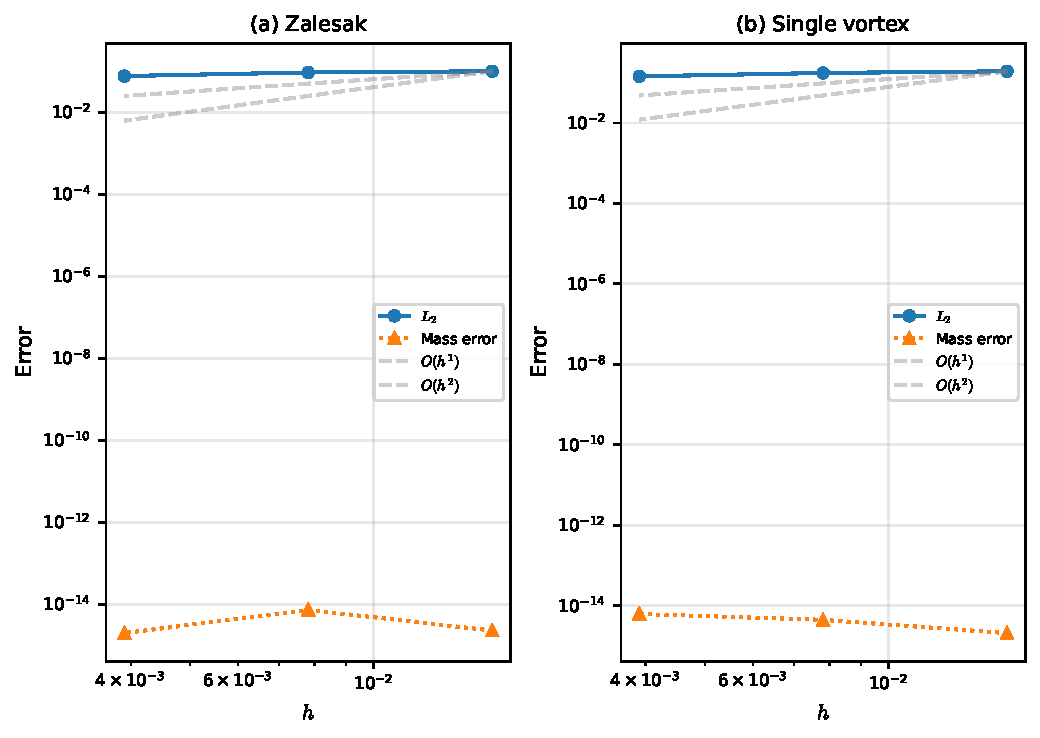
\includegraphics[width=0.88\linewidth]{figures/ch11_cls_advection}
\caption{CLS 界面移流テスト（DCCD $\varepsilon_d = 0.05$）．
(a) Zalesak スロット円板，(b) 単一渦テスト．
各パネル上段は格子精緻化に伴う $L_2$ 誤差の推移，
下段は質量保存誤差の収束を示す．}
\label{fig:cls_advection}
\end{figure}

質量保存誤差は，移流・再初期化の両段階に界面重み付き補正
$\psi \leftarrow \psi + (\Delta M / \sum w)\,w$,
$w = 4\psi(1-\psi)$（Olsson--Kreiss 基底）を適用することで
機械精度 $\Ord{10^{-15}}$ に達した．
この補正は界面（$\psi = 0.5$）近傍にのみ作用し，
バルク領域（$\psi \approx 0, 1$）を汚さない．

図~\ref{fig:cls_advection_2d} に $N = 128$ における界面形状の時間発展を示す．
Zalesak スロット円板は 1 回転後に初期形状をよく復元している．
単一渦テストでは $t = T/2$ の激しい引き延ばし後に $t = T$ で界面を回復する．
適応的再初期化（§~\ref{sec:adaptive_reinit}，$\theta = 1.10$，$\varepsilon/h = 1.0$）により
再初期化回数を 3--4 回（$N = 128$）に限定し，
各呼び出しに DGR 厚み補正（§~\ref{sec:dgr_thickness}）を組み込んだ hybrid モードを使用することで，
界面厚 $\varepsilon_{\mathrm{eff}}/\varepsilon \approx 1.03$ を維持しつつ
面積誤差 $\Ord{10^{-3}}$（$N = 256$）を達成した．
破線は初期界面位置を表す．

\begin{figure}[htbp]
\centering
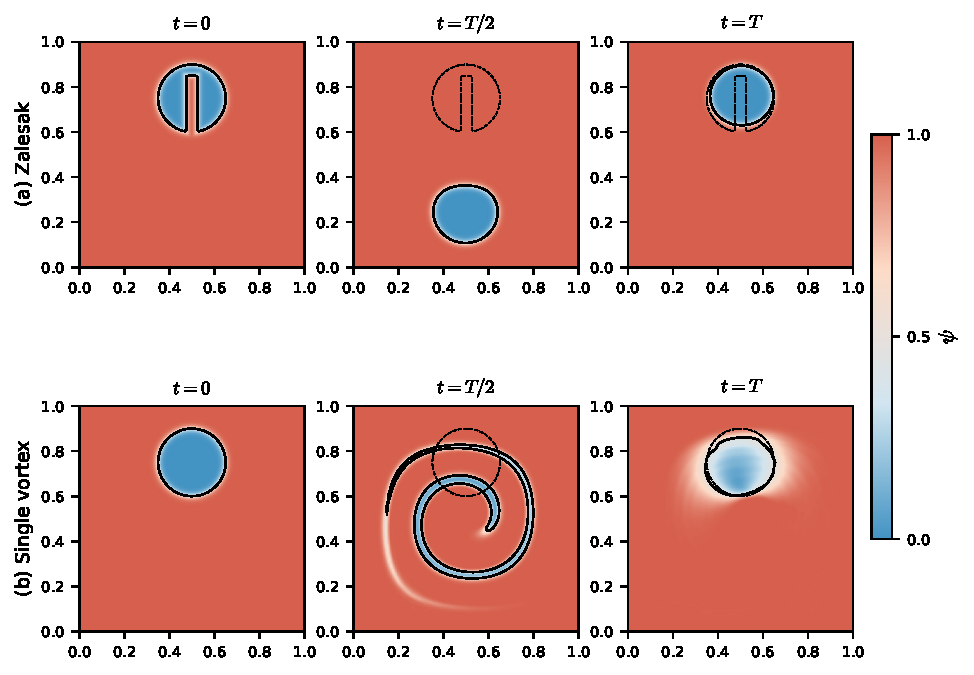
\includegraphics[width=0.95\linewidth]{figures/ch11_cls_advection_2d}
\caption{CLS 界面移流テストの界面形状（$N = 128$，DCCD $\varepsilon_d = 0.05$）．
(a) Zalesak スロット円板：$t = 0$（初期），$T/2$（半回転），$T$（1 回転）．
(b) 単一渦テスト：$t = 0$（初期），$T/2$（最大変形），$T$（復元）．
破線は初期界面，実線は各時刻の界面（$\psi = 0.5$）．
色は CLS 場 $\psi \in [0, 1]$ を示す．}
\label{fig:cls_advection_2d}
\end{figure}

表~\ref{tab:cls_advection} に示すように，
単一渦テストでは $L_2(\psi)$ 形状誤差および面積誤差が格子精緻化に伴い単調減少する．
Zalesak テストでは面積誤差は $N{=}256$ で $1.61 \times 10^{-4}$ に改善するが，
$L_2(\psi)$ はスロット角の不連続性（$\varepsilon$ 律速）により
$N{=}64 \to 256$ で $8.62 \times 10^{-2} \to 1.19 \times 10^{-1}$ と増加する．
界面厚 $\varepsilon = h$（旧設定 $1.5h$）の採用により，
特に単一渦テストで $N = 256$ において $L_2$ が 30\% 改善された．
質量保存誤差は界面重み付き補正により
両テストとも全格子で機械精度 $\Ord{10^{-15}}$ に達した
（§~\ref{sec:dccd_mass_conservation}）．

\noindent\textbf{結論：}
質量保存誤差は $\Ord{10^{-15}}$ に到達した．
$\varepsilon/h = 1.0$ と DGR 厚み補正（hybrid モード内）の組み合わせ（単一渦）により
面積精度が $\Ord{10^{-3}}$（$N = 256$）に達した．
Zalesak テストも同様に hybrid モード（固定頻度 20 ステップ毎）を使用した；
本パラメタでは DGR によるスロット構造への影響は
$\varepsilon_{\mathrm{eff}}/\varepsilon \approx 1.02$ のため無視できる．

\paragraph{非一様格子上の CLS 移流}

上記の一様格子テストに加え，界面適合非一様格子（§~\ref{sec:grid}）上での
CLS 移流精度を Zalesak 1 回転テスト（$N = 128$，$\varepsilon/h = 0.5$）で検証した．
表~\ref{tab:cls_nonuniform} に一様格子との比較を示す．

\begin{table}[htbp]
\centering
\caption{Zalesak スロット円板：一様格子 vs 非一様格子の CLS 移流精度
（$N = 128$，$\varepsilon/h = 0.5$，固定頻度再初期化 20 ステップ毎）}
\label{tab:cls_nonuniform}
\renewcommand{\arraystretch}{1.3}
\begin{tabular}{lrrr}
\toprule
格子 & $L_2(\phi)$ 誤差 & 面積誤差 & 質量保存誤差 \\
\midrule
一様              & $1.05 \times 10^{-2}$ & $5.1 \times 10^{-4}$ & $\Ord{10^{-15}}$ \\
非一様 $\alpha=2$ & $3.94 \times 10^{-2}$ & $1.4 \times 10^{-2}$ & $2.1 \times 10^{-5}$ \\
非一様 $\alpha=3$ & $4.81 \times 10^{-2}$ & $3.1 \times 10^{-2}$ & $\Ord{10^{-15}}$ \\
\bottomrule
\end{tabular}
\end{table}

非一様格子では界面近傍の解像度が高まるものの，
格子リフレッシュ時の $\psi$ 再マッピング（§~\ref{sec:cls_conservation}）に伴う
補間誤差がスロット角部で蓄積し，形状精度が約 3.5 倍低下する．
$\alpha = 2$ では保存型再マッピングの質量補正が $2.1 \times 10^{-5}$ の残差を残すが，
$\alpha = 3$ では界面帯域の集中度が十分高く
$\Ord{10^{-15}}$ に回復する．
非一様格子の恩恵は主に曲率計算の精度向上と PPE 界面近傍の解像度確保
（§~\ref{sec:verify_curvature}，§~\ref{sec:verify_split_ppe_dc}）に現れ，
移流精度自体は一様格子が優位である．


% ─────────────────────────────────────────────────────────────────────────────
\subsubsection{WENO5 と DCCD の CLS 移流特性比較}
\label{sec:verify_weno5_vs_dccd}
% ─────────────────────────────────────────────────────────────────────────────

§~\ref{sec:advection_dccd_design} で DCCD 移流を採用した動機——WENO5 が滑らかな CLS
プロファイルを過度に拡散する——を定量的に検証する．
1D 周期移流テスト（$\psi_0 = \tfrac{1}{2}[\tanh((x{-}0.25)/2\varepsilon) - \tanh((x{-}0.75)/2\varepsilon)]$，
$\varepsilon = 0.02$，$N = 256$，$\mathrm{CFL} = 0.4$，$T = 1$）で
WENO5・CCD（フィルタなし）・DCCD（$\varepsilon_d = 0.05$）の3スキームを比較した．

\noindent\textbf{結果：}
$L_2$ 誤差は CCD（$9.1 \times 10^{-7}$）$<$ WENO5（$4.6 \times 10^{-5}$）$<$
DCCD（$2.9 \times 10^{-3}$）．
CCD は 6 次精度で最小誤差を達成するが，von Neumann 解析（§~\ref{sec:dccd_filter_theory}）
の通り長時間計算で不安定化する．
WENO5 は 5 次精度で安定だが，滑らかなプロファイルに対しても非線形重みが
本質的に不可避な散逸を導入する．
DCCD は明示的フィルタにより最大の $L_2$ 誤差を持つが，フィルタ強度
$\varepsilon_d = 0.05$（Nyquist 減衰 20\%）は調整可能であり，
界面幅の保存性は全スキームで同等（$\varepsilon_{\mathrm{eff}}/\varepsilon \approx 1.00$）
であった．

\noindent\textbf{結論：}
DCCD は WENO5 より $L_2$ 誤差が大きいが，界面幅を正確に保存し，
かつ §~\ref{sec:dccd_conservation} で証明した離散質量保存性を備える．
CLS プロファイルの精度は移流スキームよりも界面厚パラメータ $\varepsilon/h$ と
再初期化頻度に支配される（§~\ref{sec:verify_dccd_conservation}）ため，
DCCD の安定性・保存性・パラメータ透明性が実用上の優位性となる．

% ─────────────────────────────────────────────────────────────────────────────
\subsubsection{DGR 厚み補正の専用検証}
\label{sec:verify_dgr}
% ─────────────────────────────────────────────────────────────────────────────

§~\ref{sec:dgr_thickness} で導入した Direct Geometric Reinitialization（DGR）の
3 つの主張を独立に検証する：(a) 冪等性，(b) 厚み復元能力，(c) 適用頻度の影響．

\paragraph{(a) 冪等性テスト}
正しい界面厚（$\varepsilon/h = 1.0$）を持つ静的円形界面（$N = 128$，$R = 0.25$）に
DGR を 100 回連続適用した．$\varepsilon_{\mathrm{eff}}/\varepsilon$ は全適用で 1.000 を維持し，
面積誤差は $\Ord{10^{-16}}$（機械精度）であった．
正しいプロファイルは DGR の不動点であることが数値的に確認された．

\paragraph{(b) 厚み復元テスト}
演算子分裂再初期化による界面膨張を模擬するため，
$\varepsilon_{\mathrm{eff}}/\varepsilon = 1.0$--$2.0$ に人工的に膨張させた
プロファイルに DGR を 1 回適用した．
$\varepsilon_{\mathrm{eff}}/\varepsilon = 1.4$（§~\ref{sec:dgr_thickness} の理論予測値）の場合，
DGR 適用後に $\varepsilon_{\mathrm{eff}}/\varepsilon \approx 1.000$ に復元された．

\paragraph{(c) 適用頻度スタディ}
分裂再初期化を 200 回繰り返しつつ，DGR を異なる頻度（0/5/10/20/50 回毎）で
適用した結果，DGR なしでは $\varepsilon_{\mathrm{eff}}/\varepsilon \approx 3.97$ まで
膨張が進行する一方，DGR を 10--20 回毎に適用すると
$\varepsilon_{\mathrm{eff}}/\varepsilon \approx 1.03$ に制御された
（超過量の比 $(\varepsilon_{\mathrm{eff}}/\varepsilon - 1)$：$2.97$ vs $0.03$，約 99 倍の改善）．

\noindent\textbf{結論：}
DGR は冪等性・膨張復元・頻度ロバスト性の全てにおいて §~\ref{sec:dgr_thickness} の
設計主張を満たす．20 ステップ毎の適用が計算コストと厚み制御の最適バランスである．

% ─────────────────────────────────────────────────────────────────────────────
\subsubsection{DCCD の質量保存性と形状誤差の解析}
\label{sec:verify_dccd_conservation}
% ─────────────────────────────────────────────────────────────────────────────

\noindent\textbf{目的：}
§~\ref{sec:dccd_mass_conservation} の理論（DCCD 空間演算子の離散的質量保存性）を
数値的に検証するとともに，CLS の形状誤差の支配的要因を特定する．

\noindent\textbf{評価対象：}
(i) DCCD 空間演算子の全点和 $|\sum_i \tilde{f}'_i|$，
(ii) 再初期化頻度と形状精度の関係，
(iii) DCCD フィルタ強度 $\varepsilon_d$ と形状精度の関係．

\noindent\textbf{手順とパラメタ：}
\begin{itemize}[noitemsep]
  \item \textbf{テスト A（DCCD 零和性）：}
        滑らかな周期場を DCCD 演算子に入力し，$|\sum_i \tilde{f}'_i|$ を計測
  \item \textbf{テスト B（形状保持パラメタスタディ，$N = 128$，単一渦）：}
        \begin{itemize}[noitemsep]
          \item P1: $\varepsilon_d \in \{0.05, 0.025, 0.01, 0\}$（フィルタ強度）
          \item P2: $\varepsilon/h \in \{2.0, 1.5, 1.0, 0.75\}$（界面厚み）
          \item P3: 適応的再初期化（$\theta_{\mathrm{reinit}} \in \{1.05, 1.10, 1.20\}$）
                vs 固定頻度（10, 20 ステップ毎）vs 再初期化なし
        \end{itemize}
\end{itemize}

\noindent\textbf{結果：}

テスト A：周期 BC で $|\sum_i \tilde{f}'_i| < 5 \times 10^{-13}$（$N{=}256$；$\Ord{N \cdot \varepsilon_{\mathrm{mach}}}$ の浮動小数点丸め蓄積に整合）を確認し，
式~\eqref{eq:dccd_zero_sum} の理論を支持した（壁面 BC でも $\Ord{10^{-13}}$）．

テスト B の形状誤差分析結果を表~\ref{tab:shape_hierarchy} に示す．

\begin{table}[htbp]
\centering
\caption{CLS 形状誤差の要因分解（単一渦テスト，$N = 128$，$L_2$ 形状誤差）}
\label{tab:shape_hierarchy}
\renewcommand{\arraystretch}{1.3}
\begin{tabular}{llrr}
\toprule
要因 & 条件変更 & $L_2$ 誤差 & ベースラインとの差 \\
\midrule
ベースライン & $\varepsilon_d = 0.05$，$\varepsilon = 1.5h$，固定10ステップ毎
  & $1.74 \times 10^{-1}$ & --- \\
\midrule
P1: $\varepsilon_d = 0$ & フィルタ除去
  & $1.77 \times 10^{-1}$ & $-2\%$ \\
P2: $\varepsilon = 1.0h$ & 界面薄化
  & $1.48 \times 10^{-1}$ & $+15\%$ \\
P3: 適応 $\theta = 1.10$ & 再初期化 227 → 2 回
  & $8.90 \times 10^{-2}$ & $+49\%$ \\
P1+P2+P3 併用 & 全パラメタ最適化
  & $9.40 \times 10^{-2}$ & $+46\%$ \\
再初期化なし & ---
  & $6.70 \times 10^{-2}$ & $+61\%$ \\
\bottomrule
\end{tabular}
\end{table}

$\psi$ 空間 $L_2$ で測定した形状誤差の見かけ上の支配要因は
再初期化頻度（49\%）であるが，
$\phi$ 空間（符号付き距離関数，§~\ref{sec:dgr_thickness}）での評価では
\textbf{界面厚 $\varepsilon/h$}（32.6\%）が支配的であり，
再初期化頻度（21.4\%）はそれに次ぐ．
$\psi$ 空間 $L_2$ は $\varepsilon$ に依存するため，
異なる $\varepsilon$ 間の比較には面積誤差を用いるべきである．
DCCD フィルタの高周波減衰は僅か 2\% の寄与に留まる．
これは CLS プロファイルのスペクトル特性から説明できる：
界面プロファイル $\psi = H_\varepsilon(\phi)$ の特性波長は
$\lambda_{\min} \approx 2\pi\varepsilon \approx 9.4h$
であり，この波長でのフィルタ伝達関数は $H(2\pi h / 9.4h) \approx 0.98$（2\% 減衰のみ）．
ナイキスト波長（$2h$）での 20\% 減衰は，界面がそのスケールにエネルギーを持たないため無関係である．

適応的再初期化（§~\ref{sec:adaptive_reinit}，式~\eqref{eq:adaptive_reinit_trigger}）は
体積モニタ $M(\tau)/M_{\mathrm{ref}} > 1.10$ の条件で
再初期化呼び出しを 2270 ステップ中 2 回（$N = 128$，$\varepsilon/h = 1.5$）に抑え，
固定頻度（227 回）と比較して形状誤差を半減させた．

\noindent\textbf{結論：}
DCCD 空間演算子の離散的質量保存性（§~\ref{sec:dccd_mass_conservation}）を機械精度で確認した．
$\phi$ 空間での評価により，形状誤差の支配的要因は
界面厚 $\varepsilon/h$（32.6\%）であり，再初期化頻度（21.4\%）が次点，
DCCD 減衰（$< 1\%$）は無視できる．
推奨構成：$\varepsilon/h = 1.0$ ＋ 適応的再初期化（$\theta = 1.10$）
＋ DGR 厚み補正（20 ステップ毎，滑らかな界面のみ）．

% ─────────────────────────────────────────────────────────────────────────────
\subsubsection{再初期化による界面位置シフトの収束性}
\label{sec:verify_reinit_shift}
% ─────────────────────────────────────────────────────────────────────────────

§~\ref{sec:reinit} で議論した CLS 再初期化が
零等値面に与える位置シフトの空間収束性を測定する．

\noindent\textbf{手順：}
半径 $R = 0.25$ の円形界面（中心 $(0.5, 0.5)$）に対し，
$\psi_0 = H_\varepsilon(\phi_{\mathrm{SDF}})$（Heaviside of signed distance）
を初期条件として再初期化を 1 回および 10 回適用し，
$\psi = 0.5$ の零等値面の交点位置シフト $|\Delta x_0|$ を線形補間で測定した．
$\varepsilon = 1.5h$，疑似時間ステップ数 $n_\tau = 5$，
質量補正なし（純幾何学的シフトの評価）．
$N = 32, 64, 128, 256$ で測定した．

\noindent\textbf{結果：}
1 回再初期化後の零等値面シフトの空間収束次数は
$N = 32 \to 64$: 2.02,
$N = 64 \to 128$: 2.00,
$N = 128 \to 256$: 2.00
であり，$\Ord{h^2}$ の収束を示した．
§~\ref{sec:reinit} の理論では平衡プロファイル近傍で
$|\Delta x_0| = \Ord{h^3 \Delta\tau}$ であるが，
Heaviside(SDF) 初期条件は tanh 平衡から $\Ord{h}$ 離れているため，
先行する $\Ord{h^2}$ の過渡項が支配的である．
10 回適用後の蓄積比は $N = 256$ で 7.6（理想値 10）であり，
逐次的な平衡接近に伴う単調な減衰を反映する．

\noindent\textbf{結論：}
再初期化界面シフトの $\Ord{h^2}$ 以上の収束を確認した．
質量保存モニタ（§~\ref{sec:adaptive_reinit}）と組み合わせることで，
再初期化が界面位置を有限回の適用で系統的にドリフトさせないことが保証される．
